\documentclass{standalone}
\usepackage{tikz}
\usepackage{ctex,siunitx}
\setCJKmainfont{Noto Serif CJK SC}
\usepackage{tkz-euclide}
\usepackage{amsmath}
\usetikzlibrary{patterns, calc}
\usetikzlibrary {decorations.pathmorphing, decorations.pathreplacing, decorations.shapes,}
\begin{document}
\small
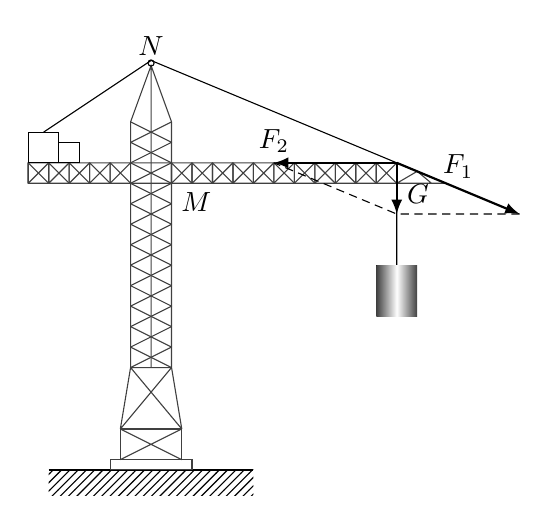
\begin{tikzpicture}[>=latex,scale=1.3]
  % \useasboundingbox (-0.1,0.1) rectangle(6,-3);
  \draw[thick](-3.4,-3)--(-1.4,-3);
  \fill[pattern=north east lines](-3.4,-3.25)rectangle(-1.4,-3);
  \draw[darkgray](-2.8,-3)rectangle(-2.0,-2.9);
  \draw[darkgray](-2.7,-2.9)rectangle(-2.1,-2.6);
  \draw[darkgray](-2.7,-2.9)--(-2.1,-2.6)(-2.7,-2.6)--(-2.1,-2.9);
  \draw[darkgray](-2.7,-2.6)--(-2.2,-2.0)(-2.6,-2.0)--(-2.1,-2.6)(-2.7,-2.6)--(-2.6,-2.0)(-2.2,-2.0)--(-2.1,-2.6)(-2.4,0.95)--(-2.4,-2.0)(-2.6,0.4)--(-2.6,-2.0)--(-2.2,-2.0)--(-2.2,0.4)--(-2.4,0.95)node[above,text=black]{$N$}--(-2.6,0.4);
  \draw(-2.4,0.975)circle(0.03);
  \foreach \x in {-2,-1.6,...,0}
  {
    \draw[darkgray,line join=round](-2.6,\x)--(-2.2,\x+0.2)--(-2.6,\x+0.4);
    \draw[darkgray,line join=round](-2.2,\x)--(-2.6,\x+0.2)--(-2.2,\x+0.4);
  }
  \draw[darkgray](0.48,-0.2)--(-3.6,-0.2)(0,0)--(-3.6,0)--(-3.6,-0.2)(0,-0.2)--(0.2,-0.083)--(0.34,-0.2);
  \foreach \x in {0,-0.2,...,-2.0,-2.6,-2.8,...,-3.4}
  {
    \draw[darkgray,line join=round](\x,0)--(\x-0.2,-0.2)--(\x-0.2,0);
    \draw[darkgray,line join=round](\x,-0.2)--(\x-0.2,0)--(\x-0.2,-0.2);
  }
  \draw(0.48,-0.2)--(-2.4,1.0)(0,0)--(0,-1)(-2.4,1.0)--(-3.45,0.3);
  \draw[thick,->](0,0)--(1.2,-0.5)node[midway,above]{$F_1$};
  \draw[thick,->](0,0)--(-1.2,-0)node[above]{$F_2$};
  \draw[thick,->](0,0)--(0,-0.5)node[above right]{$G$};
  \draw[thin,densely dashed](1.2,-0.5)--(0,-0.5)--(-1.2,0);
  \fill[left color=darkgray,right color=darkgray,middle color=white](-0.2,-1)rectangle(0.2,-1.5);
  \draw(-3.6,0)rectangle(-3.3,0.3)(-3.3,0.0)rectangle(-3.1,0.2);
  \node at (-2.2,-0.2)[below right]{$M$};
\end{tikzpicture}
\end{document}